%-----------------------------------------------------------------------------
%
%               Template for sigplanconf LaTeX Class
%
% Name:         sigplanconf-template.tex
%
% Purpose:      A template for sigplanconf.cls, which is a LaTeX 2e class
%               file for SIGPLAN conference proceedings.
%
% Guide:        Refer to "Author's Guide to the ACM SIGPLAN Class,"
%               sigplanconf-guide.pdf
%
% Author:       Paul C. Anagnostopoulos
%               Windfall Software
%               978 371-2316
%               paul@windfall.com
%
% Created:      15 February 2005
%
%-----------------------------------------------------------------------------


\documentclass{sigplanconf}

% The following \documentclass options may be useful:

% preprint      Remove this option only once the paper is in final form.
% 10pt          To set in 10-point type instead of 9-point.
% authoryear    To obtain author/year citation style instead of numeric.

\usepackage{amsmath}
\usepackage{listings}
\usepackage{graphicx}

\begin{document}

\special{papersize=8.5in,11in}
\setlength{\pdfpageheight}{\paperheight}
\setlength{\pdfpagewidth}{\paperwidth}

\conferenceinfo{CONF 'yy}{Month d--d, 20yy, City, ST, Country} 
\copyrightyear{20yy} 
\copyrightdata{978-1-nnnn-nnnn-n/yy/mm} 
\doi{nnnnnnn.nnnnnnn}

% Uncomment one of the following two, if you are not going for the 
% traditional copyright transfer agreement.

%\exclusivelicense                % ACM gets exclusive license to publish, 
                                  % you retain copyright

%\permissiontopublish             % ACM gets nonexclusive license to publish
                                  % (paid open-access papers, 
                                  % short abstracts)

\titlebanner{banner above paper title}        % These are ignored unless
\preprintfooter{short description of paper}   % 'preprint' option specified.

\title{Refactoring towards Cloud-enabled Multiuser Mobile Apps}

\authorinfo{Arpit Christi }
           {Oregon State University}
           {chrsitia@eecs.oregonstate.edu}
\authorinfo{Michael Hilton}
           {Oregon State University}
           {hiltonm@eecs.oregonstate.edu}
\authorinfo{Danny Dig}
           {Oregon State University}
           {digd@eecs.oregonstate.edu}
\authorinfo{Michal Moskal}
           {Microsoft Research}
           {Michal.Moskal@microsoft.com}
\authorinfo{Sebastian Burckhardt}
           {Microsoft Research}
           {sburckha@microsoft.com}
\authorinfo{Nikolai Tillmann}
           {Microsoft Research}
           {nikolait@microsoft.com}
\maketitle


\begin{abstract}
Cloud computing has become a great tool for many developers to use, with many benefits, especially in mobile development.  However, adding cloud functionality to an existing app can be difficult and time-consuming. We present \textsc{cloudifyer}, a tool that can automatically refractor \emph{local} data structures into \emph{cloud} data structures on the TouchDevelop platform.  As this platform targets students and hobbyist programmers, lowering the barrier of entry to using the cloud is imperative.
\end{abstract}


\section{Introduction}
% mobile is everywhere. mobile cloud computing can make it better. Examples

% What's broken: advanced expertise, infrastructure, multiple languages

% In this paper we want to lower the entry barrier for developers, so that even hobbyists and beginner mobile app devs. Thus, TouchDevelop + Refactoring

% Intro to TouchDevelop and its cloud datatype

% our formative study to learn about refactorings from single to multi-user apps. refactorings for data structures

% Automated refactoring based on these lessons, why do we need refactoring support.

% Contributions
This paper makes the following contributions:


Cloud computing has been a long held dream of treating computing as a utility~\cite{Armbrust:2010:VCC:1721654.1721672}.  It can enable developers with innovative ideas for new Internet services to no longer require the large capital outlays in hardware to deploy their service, or human expense to operate it.  By using a pay-as-you-go pricing model, resources are only paid for if they are needed, which lowers the up-front investment, and allows developers to avoid paying for unneeded resources~\cite{zhang2010cloud}.  Some examples of cloud computing servers include Amazon EC2, Windows Azure, and Google App Engine.  While there are many benefits of cloud computing, there are also some disadvantages. As cloud services are often remote, they can suffer from latency and bandwidth related issues~\cite{4804045}.  This provides a challenge to developers if they wish to provide a similar experience to users while still taking advantage of the benefits that cloud computing can offer.  In addition, if a developer wishes to transform an existing application that previously had only dealt with data locally, there new must be a new communication layer that the developer must deal with 
in order to transform the application to use cloud services.  

If a programmer decides to set up a cloud server, they will first have to determine the candidate data structures and candidate methods that operate on data structures to move to the cloud server. Then the programmer will have to program the desired functionality to run on the cloud server.  Often this will involve using a completely different language and environment as the rest of the application.  Some common technologies for communicating with the remote application are web services, REST services and WCF services. Building services using any of these technologies require the programmer to learn IDEs and programming languages that support these technologies.

 Once the programmer is able to build a service to run on the cloud server, they still need to execute the manual steps of moving the services to cloud. Unless the programmer has access to a cloud server, they will most likely have to use a commercial service such as Amazon EC2 or Windows Azure. The programmer will also have to develop a way to persist the data on the cloud server.  This would involve learning how to use cloud data storage such as Amazon S3 or Microsoft SkyDrive.  Performing all these steps is clearly a challenge even for an experience user, as all these steps are manual, time consuming, error prone and may require multiple iterations of them before reaching a stable error free level.
  
TouchDevelop~\cite{Tillmann2011TPC20482372048245} is a programming environment and language developed by Microsoft Research which makes it possible to write applications on mobile devices.  TouchDevelop was designed to engage users by allowing them to write scripts that show and manipulate items that connect with their personal interests and possessions, such as music and pictures on their phone, the sensors of the phone, and the friends in their social networks.  TouchDevelop includes a typed, structured programming language that is built around the idea of only using a touchscreen as the input device to develop code.  It has built in primitives that make it easy to access common sensors on mobile devices.  While the language is similar to traditional text-based languages, the editor has enforced structure to help avoid syntax errors as users will be entering their data with the less than precise touch gestures.
  
Before the introduction of cloud types, TouchDevelop supported REST calls to web services.  This allowed users to connect to an existing REST server and add functionality to their application.  However, if the REST server did not already exist, setting up such a server would involve a significant amount of knowledge and effort.  As TouchDevelop's target audience includes students and hobbyist programmers~\cite{Tillmann2011TPC20482372048245}, this would almost certainly be more then could be reasonably expected from them.  

In order to assist developers with introducing cloud functionality into their scripts, TouchDevelop introduced specialized cloud data types.~\cite{burckhardt2012cloud}  These cloud types were designed to provide an abstraction layer to free developers from concerns such as web service implementation, communication protocols, and local storage.  In order to make the app responsive, even when the connection to the server is unavailable, cloud data types provide both local copies of the data as well as eventually constant sharable cloud storage.   This implementation allows programmers to use cloud types in a similar manner to local data structures, but to also enjoy the benefits of the cloud.

To enable TouchDevelop programmers to take advantage of these new features, we designed, implemented and evaluated  \textsc{cloudifyer}, a novel tool that will perform refactorings from local data types to cloud data types in an automated manner. As far as we know, this is the first tool to perform then entire refactoring from local data to cloud data automatically.
The rest of the paper is structured as follows.  Section~\ref{sec:motivatingExample} presents a motivating example for this refactoring.  Section~\ref{sec:TouchDevelop} provides an overview of the TouchDevelop platform as well as some of the cloud data type implementation details.  Section~\ref{sec:Refactoring} describes the refactoring that we implemented.  Section ~\ref{sec:evaluation} presents the results of evaluating \textsc{cloudifyer} by running it on 109 existing touch develop scripts, of which we were able to refactor 88\%.  For every refactoring we were able to perform an average of 11 transformations to each script in 9 seconds. We present a discussion of related work in Section~\ref{sec:relatedWork}.  We finish the paper in Section~\ref{sec:conclusions} with our conclusions and future work.


\section{Motivating Example}
\label{sec:motivatingExample}
In this section we introduce a motivating example for refactoring data structures to the cloud.   Consider a program called Mileage Tracker that allows the user to store their milage so that they can be aware of their fuel usage.  The user can input how much gas was needed to fill his tank, as well as the miles driven since the last fill up.  This allows the application to be able to calculate what was the miles per gallon since the last fill up.  The script will store this information and allow the user to view their fuel usage over time.  This application was written before the introduction of cloud data to the TouchDevelop platform, and so the way that the application was developed, the data was being stored locally in a local data structure.  The developer did check the option which preserves the values of the data structure across multiple runs, so as long as user uses same device, he will have up to date information regarding its mileage usage.  However, the script cannot work across multiple devices which does not support the ability for multiple family members using the same family car to share their information effectively.


\subsection{Goals of Refactoring to Cloud}
The developer of the MPG tracking application would like to take advantage of cloud functionality.  Specifically, the developer would like to enable the users to be able to access their data on multiple devices and see the same data. The developer would also like to enable social, collaborative features such as allowing users to share their MPG values with other users of the app.

This program was written before the introduction of the cloud API's to the TouchDevelop language.  The program does not use any cloud data types, and all data is stored locally.

Before the introduction of the cloud data types, the developer could select the "save between script runs" option for local data, which would persist the data structures across multiple runs of the script.  This approach has several limitations which significantly reduce the usefulness of the application to the end user.  One of the major limitations of this approach is that the information can not be synced between devices.  The user would only be allowed to track their MPG's on one single device.  This poses a problem if the user would like to upgrade their device,or if there phone was lost or broken.   Also, this approach will not work if there are multiple drivers of the vehicle, and they would like to be able to collaborate on tracking their fuel efficiency.  However, this would not be possible using the local data structure.


  
\subsection{Problem}
If the application had been developed using the TouchDevelop table data structure, converting to a cloud table is a trivial operation.  It is as simple as selecting the table object and changing the type to cloud table.  The refactoring becomes non-trivial if the user was using another data structure, such as a collection. A TouchDevelop collection is a data structure that consists of a collection of any type of object that TouchDevelop supports.  This could be a primitive type such as Number or String, or it could be something as complex as a Camera object, or a Map object.  The difficulty in refactoring an existing collection into a cloud data structure arises in the need to convert into a cloud table.  The methods that collection provides and the methods that cloud table provides have some overlap, but are not consistent.  In addition, there are methods for \textsc{number collection} that have no counterpart for cloud table, i.e. avg.  Table~\ref{tab:mappingTable} shows the operations that are available for \textsc{number collection}s, as well as the corresponding operations for cloud table, if they exist.  We have categorized the type of transformation that will be necessary to transform every possible collection operation into a cloud table operations.  We will describe how we perform these transformations Section~\ref{sec:Refactoring}.

\begin{table*}[htb!]
\centering
\begin{center}
\begin{tabular}{|c|c|c|}
 \hline
Number Collection Operations & Cloud Table Operations & Transformation Type\\
 \hline
  \hline
add & add row & Indirect \\ 
\hline
at & row at & Indirect \\
\hline
add many() & NONE & Function \\
\hline
avg & NONE & Function \\
\hline
clear & clear & Direct \\
\hline
contains & NONE & Function \\
\hline
count & count & Direct \\
\hline
index of &NONE  & Function \\
\hline
insert at & row at$\rightarrow$value & Indirect \\
\hline
max &NONE  & Function \\
\hline
min & NONE & Function \\
\hline
post to wall & post to wall & direct \\
\hline
random &NONE  & Function \\
\hline
remove  & NONE & Function \\
\hline
remove at & row at()$\rightarrow$deleteRow & Indirect \\
\hline
reverse &NONE  & Function \\
\hline
set at & row at()$\rightarrow$valueName & Indirect \\
\hline
sort & NONE & Function \\
\hline
sum & NONE & Function \\
\hline

\end{tabular}
\nocaptionrule
\caption{Table with the Number Collection API's and corresponding Cloud Table Operations}
\label{tab:mappingTable}
\end{center}
\end{table*}%


\section{TouchDevelop}
\label{sec:TouchDevelop}
In this section we provide a brief overview of the TouchDevelop language, as well as some more discussion on how cloud data types are implemented.

\subsubsection{Cloud Data Types}
The cloud types implemented in TouchDevelop include both simple types, cloud integers, cloud strings, as well as the structured types of cloud arrays and cloud entities.   The only way that these cloud types are exposed to developers is as cloud tables and cloud indexes.  The cloud table can be used in a similar manner as the local table data structure.  However, when a developer uses the cloud table, they also get an eventually consistent cloud version and the option to share the data across multiple users.

If the developer wished to take advantage of the cloud features for primitive data, they must encapsulate them into a table first.  Table~\ref{table:supportedTypes} lists the types of primitives that are allowed as column types of the cloud table.

\begin{table*}[htb!]
\begin{center}
\begin{tabular}{lcl}
  Supported Cloud \\
  Table Types  \\
   \hline
Boolean  \\
Number \\
String  \\
DateTime  \\
Location  \\
User  \\
\end{tabular}
\nocaptionrule
\caption{Supported Types}
\label{table:supportedTypes}
\end{center}
\end{table*}%



\subsubsection{sessions}
There are two different types of cloud sessions that are offered by TouchDevelop.  There is the default session, called the "just-me" session as well as the "everyone" session.  \subsubsection{just-me session}
The "just-me" session is meant to share data between all devices by the same user running the same script.  Other users cannot connect to this session.  When the MPG script is refactored to use the just-me session, the user will now have the opportunity to see all of their data regardless of which device they are on. This allows the user to have the application installed on their phone and tablet and to share the data across each. 

\subsubsection{everyone session}
The "everyone" session creates a session that everyone running the script can connect to.  All users of the script will see the same data.  For the MPG example, the everyone session would allow users to see the MPG statistics of a community of users.  All users would add their MPG data to the common table, and the statistics that they would see would be for the entire community.  For example, when they see the average MPG, it would be the AVG for all the users of the script.



  
\section{DataStructure to Cloud REFACTORING}
\label{sec:Refactoring}
This section presents the data structure to cloud refactoring.  We explain \textsc{cloudifyer}'s workflow, as well as the three types of transformations that we have identified that are necessary for the refactoring. 

\subsection{Workflow}
\textsc{cloudifyer} is written in TouchDevelop, and can be run using the TouchDevelop platform.  Once it is run, the user is presented with a picker to choose which script to refactor.  This must be a script that is saved for that user, but any public script can be saved as your own script. When the user selects which script they wish to refactor, they are presented with all \textsc{number collection}s that are a part of this script.  The user can then choose which \textsc{number collection} they wish to refactor by typing in the name into a standard TouchDevelop wall prompt box. Once the user has typed in the name and clicked the ``ok'' button, the tool will automatically refactor all the calls to the selected \textsc{number collection}, and then present some output to the user, which includes how many of each type of transformation were performed, as well as the total time required to complete the refactoring. 


\subsection{Algorithm}
We describe the algorithm that is used by the refactoring engine to refactor TouchDevelop scripts.   

Step 1: Create a new Cloud Data structure that transformations will use and add it to the script.

Step 2: Traverse through the script and find candidate statements for refactoring.

Step 3: Refactor local data structure statements into corresponding cloud data structure statements.

To explain our algorithm, we will walkthrough the refactoring of a TouchDevelop script, BlockY World.  BlockY World is a game where our hero must find his way through a maze of blocks, while also being able to move blocks to change the environment around him.  BlockY World uses multiple \textsc{number collection}s named \texttt{stats}, \texttt{spestats} and \texttt{zones}. For our further discussion of algorithm, we assume that user has selected \texttt{spestats} as the \textsc{number collection} to refactor. In step 1, a cloud data type is created and injected by \textsc{cloudifyer} into the BlockY World script.  A new cloud data table is added for every refactoring to avoid conflicts if there are more then one refactoring per script. Then a column will be added to the table with the same name as the \textsc{number collection} that is being refactored.  For \texttt{spestats}, the tool will produce a cloud data table with a single column whose data type is number and who's column name is \texttt{spestats}.  In step 2, TouchDevelop's JSON AST tree representation is used to traverse script's AST. If any references to selected collection to refactor is found, the tool marks it as a candidate statement to refactor.  In step 3, each of the candidate statement is then transformed into individual new statement that replace the call to the \textsc{number collection} with a the corresponding cloud data action. 

\subsection{Transformations}
There are several categories of transformations that are needed to transform local data structures to cloud data structures.  


\subsubsection{Direct Transformations}
These are the transformations where both the \textsc{number collection} and the cloud table have the same action.  For example, both have an action "post to wall" which will, as expected, post to the scripts wall.  This is the simplest of the transformations, as all that is needed to do is replace the object that the action is being called on.  Figure~\ref{fig:numCol_postToWall} shows a line of TouchDevelop code that posts to the wall a \textsc{number collection} that is stored in the global variable named \texttt{MileageRecord}.


\begin{figure}[htbp!]
\begin{center}
\texttt{MileageRecord $\rightarrow$ post to wall}

\end{center}
\nocaptionrule
\caption{post to wall before transformation}
\label{fig:numCol_postToWall}
\end{figure}

\begin{figure}[htbp!]
\begin{center}
\texttt{Cloud Data table $\rightarrow$ post to wall}
\nocaptionrule
\caption{post to wall after transformation}
\label{fig:CloudTable_postToWall}
\end{center}
\end{figure}

Figure~\ref{fig:CloudTable_postToWall}  shows the same line of code after it has been transformed by our algorithm.  Now the cloud data table is being posted to the wall.




\subsubsection{Indirect Transformations}
The indirect transformations are slightly more complex then the direct transformations.  The indirect transformation is when there are two actions that have similar behavior, but different names.  For example, \texttt{add}, which adds to a \textsc{number collection}, and \texttt{add row} which adds to a cloud data table.  Consider the case where the user of the previous example would like to add the current mileage to the list that stores all the past mileages.  In order to add it to a \textsc{number collection}, the developer would have to use the \texttt{add} operator.  This is shown in Figure~\ref{fig:numCol_Add}.

\begin{figure}[htbp!]
\begin{center}
\texttt{MileageRecord $\rightarrow$ add(Mileage)}
\nocaptionrule
\caption{add action before transformation}
\label{fig:numCol_Add}
\end{center}
\end{figure}
\begin{figure}[htbp!]
\begin{center}
\texttt{Cloud Data table $\rightarrow$ add row $\rightarrow$ MileageRecord := Mileage}
\nocaptionrule
\caption{add action after transformation}
\label{fig:CloudTable_Add}
\end{center}
\end{figure}

Figure~\ref{fig:CloudTable_Add} shows the same line of code after it has been transformed by  \textsc{cloudifyer}.  Now the actions are operating on a cloud data table.  Since each element in the \textsc{number collection} is being mapped to a row in the cloud data table, before the number can be added a new row must be added to the table.  TouchDevelop offers the ability to chain functions together, so we can chain the add and assignment operators.  In the same line of code we can add a new row to the table, as well as set the value as the current Mileage that we wish to store.


\subsubsection{Custom Function Transformations}
The third type of transformation we have implemented is custom function transformations.  These are needed when there is no action in Cloud Table that will achieve the same functionality as the action that exits in  \textsc{number collection}. For example, the developer of the mileage tracker would like to calculate the average across all the sessions of the app.  The \texttt{avg} action will return the average of all the numbers in the \textsc{number collection}.  In order to transform a \textsc{number collection}s that contain this action, we inject a custom function into the code that provides the same behavior as the \texttt{avg} action.  Then we can transform a call from the TouchDevelop API to a call to our custom function.  Figure~\ref{fig:numCol_avg} shows a line of source code where the \texttt{avg} action is being called, and then the returned value is being stored in a local variable \texttt{avgMielage}.


\begin{figure}[htbp!]
\begin{center}
\texttt{var avgMileage := MileageRecord $\rightarrow$ avg}
\nocaptionrule
\caption{avg action before transformation}
\label{fig:numCol_avg}
\end{center}
\end{figure}

Figure~\ref{fig:CloudTable_avg_fun} shows the same line of code after \textsc{cloudifyer} has performed the transformation.  The action \texttt{Cloud Data avg} is a custom function that is generated by our refactoring engine that is needed to calculate the average of all the values in the cloud data table.  This function also returns a value, so we are saving it in the same local variable.  Figure~\ref{fig:CloudTable_avg_fun} shows the helper function that is added to the script.

\begin{figure}[htbp!]
\begin{center}
\texttt{var avgMileage := Cloud Data avg}
\nocaptionrule
\caption{avg action after transformation}
\label{fig:CloudTable_avg}
\end{center}

\end{figure}
\begin{figure}[htbp!]
\texttt{ private action Cloud Data avg()\\ 
returns(\\
avg: Number)\\
do\\
var sum := 0\\
for each ct in Cloud Data table\\
where true\\
do\\
sum := sum + ct $\rightarrow$ MileageRecord\\
avg := sum / Cloud Data table $\rightarrow$ count}
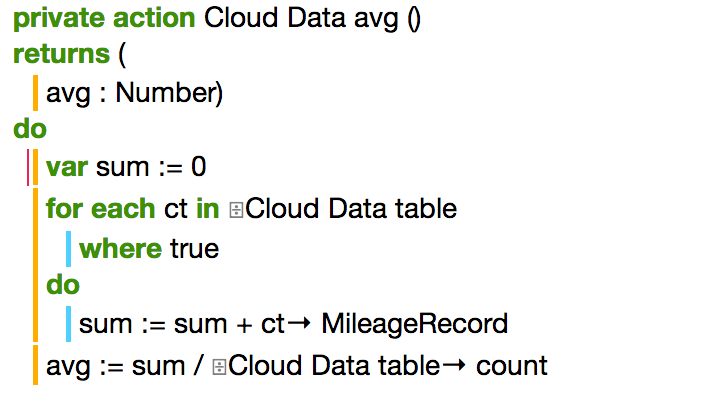
\includegraphics[width=250pt]{images/HelperFunction}
\nocaptionrule
\caption{custom function to provide avg functionality}
\label{fig:CloudTable_avg_fun}
\end{figure}

\subsubsection{Unsupported Language Features}
\label{sec:unsupportedLanguageFeatures}
There were some transformations that we were unable to perform due to limitations of the TouchDevelop language.  Local data structures, in our case the \textsc{number collection} data structure, can be passed as an input parameter (argument) or output parameter (return value) of a TouchDevelop action.  Due to language constraints, cloud data tables must be declared as global variables and cannot be used as input or output parameters.  \textsc{cloudifyer} does not attempt to perform transformation in these situations.  In the future, a transformation could potentially be developed that would transform the local structure from a parameter to a global variable, and then the local to cloud data transformation could be performed.

 \texttt{number collection}s can be assigned to a variable using the assignment operator.  However, cloud data tables are able to be assigned due to their global nature.  We are therefore unable to transform any occurrences of a data collection that use the assignment operator. 

\textsc{cloudifyer} also does not support the custom function transformation of \texttt{add many}.  We believe that this function could be implemented but it remains as future work.  For this reason,  \textsc{cloudifyer} is unable to support transformations that involve the \texttt{add many} action.



\section{Evaluation}
\label{sec:evaluation}
To determine if \textsc{cloudifyer} is useful we ask the following research questions.\\
Q1:  \textbf{APPLICABILITY}:  How applicable are the refactorings?\\
Q2:  \textbf{EFFORT}: How much effort is saved by \textsc{cloudifyer} when refactoring?\\
Q3:  \textbf{ACCURACY}: How accurate is \textsc{cloudifyer} when performing a refactoring ?\\
 
\subsection{Methodology}



\subsubsection{Verification Corpus}
We developed our refactoring tool as a TouchDevelop script.  In order to empirically evaluate the application, we ran it on 109 scripts.  In order for a script to be a candidate for refactoring it should have at least one \textsc{number collection}.  In order to make our evaluation easier, we also required the \textsc{number collection} be a global variable.  Our refactoring works on non-global variables, but using global variables simplifies the automated identification of refactoring targets.  We chose to target the top ranked scripts based on number of runs.

For each script we ran a program that would identify all the \textsc{number collection} data structures in the target script.  Once the \textsc{number collection}s had been identified, one would then be chosen to be the target of the refactoring.  For each successful refactoring we returned several metrics.

In order to determine the applicability of our tool we tracked the number of scripts that our tool was able to refactor, as well as the number of each specific class of refactoring.

In order to determine the effort saved by using this refactoring tool we record the number of seconds each refactoring took. Table~\ref{table:avgTrans} shows  the refactoring times.  The longest refactoring took 18 seconds, but the median time was only 9 seconds.  The majority of the time spent doing the refactoring was spent locating transformations, so the time that the refactoring took was correlated with the program size, not with the number of transformations performed for each script.

We did find some programs that our tool was unable to refactor.  Currently the way Cloud Data tables are implemented in TouchDevelop, they cannot be passed as arguments to a method, they may only be used as a global variable.  Since \textsc{number collection}s do have the ability to be passed as collections, the tool is unable to refactor programs where the \textsc{number collection} is passed as an argument.  We only found 5 scripts that were unable to be refactored for this reason, as noted in Table~\ref{table:totalScripts}.  We also were unable to implement the \texttt{add many} functionality, so any script that called the add many action on a \textsc{number collection} was unable to be transformed by our tool. 

In order to determine if the tool was accurate or not we chose 10 applications to manually evaluate from the list of scripts we had run our automated refactoring tool on.  In order to evaluate the accuracy we first checked to ensure that our automated tool had not introduced any new syntax errors into the script.  After that, we looked at each reference to the original \textsc{number collection} and ensured that it had been correctly transformed into the correct call to the Cloud Table.


\subsubsection{Further Validation}
In order to further validate our results we randomly chose 10 scripts to further evaluate.  We then ran the scripts for up to three minutes and explored their functionality.  During this exploration we took notes of the behavior and any output of the script.  We then performed our refactoring on each script and then ran each script for three minutes again to verify that our script had not introduced any runtime behavioral changes. We did not observe any runtime changes based on the changes to these scripts.
In addition to running these scripts we also performed code inspections of these randomly selected scripts.  We counted any potential transformations that were missed by \textsc{cloudifyer} as well as we inspected all the transformations that had been performed to see if they had been performed precisely or imprecisely.  Using these values we were able to calculate precision and recall for \textsc{cloudifyer}.  We define precision as
\[precision = \frac{|True Positive|}{|True Positive|+|False Positive|}\]
and recall as
\[recall = \frac{|True Positive|}{|True Positive|+|False Negative|}\]
A {\it TruePositive} is a potential transformation that is correctly identified as a transformation, and the transformation is correctly performed.  A {\it FalsePositive} is when \textsc{cloudifyer} applies a refactoring to a line of code that is not a potential target.  In other words, it transforms code that should not have been transformed.   {\it FalseNegative} is when a transformation that should be applied is not.  This is when \textsc{cloudifyer} does not correctly transform some code, leaving it as it was before, when in fact, it should have been transformed. 
\subsection{Results}

\textbf{APPLICABILITY}:  Table~\ref{table:totalScripts} shows the results for running our refactoring tool on 109 scripts.  Out of the 109 scripts that were attempted to be refactored by our tool, only 7 were unable to be refactored due to unsupported language features as described in Section~\ref{sec:unsupportedLanguageFeatures}.  \textsc{cloudifyer} was able to refactor 91\% of the scripts that we attempted.  This shows that \textsc{cloudifyer} is clearly applicable to a wide range of scripts that contain the \textsc{number collection} data structure.

\begin{table}[htdp]
\begin{center}
\begin{tabular}{ll}
Total Scripts & 109 \\
Number Successfully Refactored & 98 \\
Unsupported Language Features & 7 \\
Tool Crashed on Refactoring Attempt & 4\\
\end{tabular}
\nocaptionrule
\caption{Total Scripts Refactored}
\label{table:totalScripts}
\end{center}
\end{table}%

\textbf{EFFORT}:  
Figure~\ref{table:avgTrans} shows the number of transformations performed per script as well as the average times.
Each refactoring consisted on an average of almost 12 transformations.  The most common transformation was indirect transformations with 10  transformations on average for each script.

The last column shows the time in seconds.  On average each refactoring took a total of 9 seconds to complete.  The maximum length of time any single refactoring took was 18 seconds.  As the number of transformations on average was 12, this shows that our refactoring tool saves significant effort, as the time to make these transformations by hand would clearly exceed a few seconds.  
\begin{table}[htdp]
\begin{center}
\begin{tabular}{lclclclclcl}
 & Total & Direct & Indirect & Custom & Time \\
  & Trans & Trans & Trans & Function & in secs \\
  \hline
  \hline
AVG & 11.6 & 1.20 & 9.07 & 1.34 & 9.30 \\
\hline
MAX & 112 & 13 & 112 & 19 & 18 \\
\hline
\end{tabular}
\nocaptionrule
\caption{Average Transformations}
\end{center}
\label{table:avgTrans}
\end{table}%

\begin{figure}[htbp!]
\begin{center}
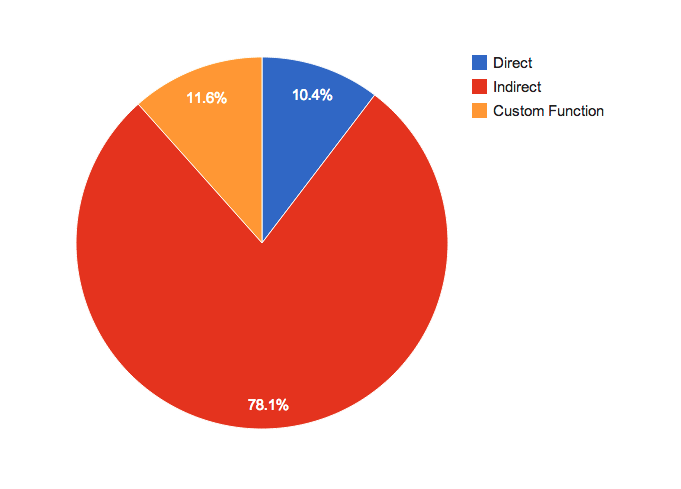
\includegraphics[width=250pt]{images/TransformationsChart}
\nocaptionrule
\caption{Transformations by Percentage}
\label{fig:transformations_pieChart}
\end{center}
\end{figure}

\textbf{ACCURACY}: By manually checking 20 scripts, we analyzed the precision and recall for our tool.  We found a precision of 100\%.  We also calculated the recall, and our recall value was 94\%. There were over 145 transformations that we inspected in these 20 scripts, and we only found 8 potential transformations that \textsc{cloudifyer} missed.

\begin{table}[htdp]
\begin{center}
\begin{tabular}{ll}

Precision & 100\% \\
Recall & 95\% \\
\end{tabular}
\nocaptionrule
\caption{Precision and Recall values}
\end{center}
\label{table:precAndRecall}
\end{table}%

\subsection{Case Studies}

\subsubsection{Motivating Example}
We forked the Mileage Tracker script and created our own Mileage Tracker script. Without making any logical change to the script, we used \textsc{number collection} instead of number map to store data. We then manually replaced a slice api call with corresponding logic as the slice api call is not available with \textsc{number collection}. We ran both the original script and our manual changes to ensure that both scripts exhibited the exact same functionality. The new Mileage Tracker script is available in TouchDevelop with script id \texttt{mfbb}.  We then refactored the Mileage Tracker script using \textsc{cloudifyer}. All the transformations were successfully applied and script did not have any compilation errors. Though to ensure that script behavior was exactly same as before we needed to make two lines of code change in InitializeApplicationSettings method of the script. As Microsoft TouchDevelop recent version removed is invalid with cloud data table, we have to replace it with corresponding logical step. The other one line of change in code is to enable everyone session on the cloud data table. This will allow multiple users with their own separate sessions to share same cloud data table. We ran the refactored Mileage Tracker application with three different devices, two laptops and one mobile phone to verify Mileage Tracker is indeed refactored into multi device, multi user application. Thus, with our automated refactorings and two lines of code changes we were successfully able to convert a single user, single device application into multi user, multi device application. The refactored Mileage Tracker Appliation is available in TouchDevelop with id \texttt{eyhca} and name Mileage Tracker Refactored. 

\subsubsection{BlockY World}
To further demonstrate the usefulness of cloud refactoring, we applied it on BlockY World, a game script written for TouchDevelop. The BlockY World script id is skdk. 65 users are following this game and the game has been installed 350.  To convert this game from single device to multi device/multi user game via refactoring, we used our tool to refactor all the collections to cloud data types. BlockY World has 8 \textsc{number collection}s and one \texttt{picture collection}. As TouchDevelop cloud data tables do not support picture type, we are unable to convert the picture collection to cloud data type.  All 8 \textsc{number collection}s were automatically refactored into corresponding cloud data type using the tool. We also added some manual code to initialize and share the data. 

However, we were unable to convert BlockY World into a multi device game.  We throughly analyzed the script to see what additional steps would be needed to complete the transition to a multiplayer game.

Our further analysis of BlockyWorld suggests that some global variables also need to be moved to cloud because to make the script multi device some global variables also need to be shared across devices over the cloud. For instance, variables like $old_x$ and $old_y$ and $curr_x$ and $curr_y$ needs to be stored across the devices. These variables are of type number.  

BlockY World consists of some variables whose cloud type representation is not available at this point of time. ercan is game board variable used for the BlockY World game. In order to effectively share the game board across multiple devices, we need to move variable ercan to cloud. Currently no cloud data type implementation supports game board variables. BlockyWorld consists many such variables whose cloud data type conversion is not possible.

We also determined that for this application, eventually consistency was not responsive enough for realtime gaming.  Though the eventual consistency model works fine with many types of applications, it is not particularly  suited for games where real time data needs to be shared quickly across device. TouchDevelop team is planning to support flush implementation for synchronization with stronger consistency model~\cite{burckhardt2012cloud}, where any changes in local data is immediately synchronized with cloud data, though it is not available currently. Though we are not able to refactor BlockY World into a multi device application through refactoring, analysis of BlockY World brought into light certain implementation level issues of both TouchDevelop as well as textsc{cloudifyer} that hinders widespread practical usage of textsc{cloudifyer} in case of realtime gaming application refactoring. 


\subsection{Threats to validity}
\textbf{Construct Validity:}  Does the evaluation of candidate scripts prove the applicability of our tool?  Since the refactoring to the cloud is such a new part of the TouchDevelop language, there is not a lot of data for us to identify when developers will actually choose to refactor to the cloud.  By showing that most of the scripts that use the local data structure are applicable candidates, we can show that there is wide applicability for our solution, should developers choose to use it or not.

\textbf{Internal Validity:}  We minimized the threat of internal validity by performing a case study of apps that were written before the introduction of Cloud Data, and by using publicly available scripts, the developers were unaware of our study.  

\textbf{External Validity:}  Do our results generalize? We chose over 100 of the most commonly run scripts to use as our corpus, but we put no restrictions on the tags, or types of the scripts.  Our selection include scripts tagged with entertainment,sports, games, education, productivity and platform bugs.  Since tags are not required in TouchDevelop we observed many scripts without tags.  However, in a addition to a wide variety of scripts tags, we also observed a variety of script types while performing the evaluations.  We do not foresee any reasons why these results would not generalize to all TouchDevelop scripts.

\textbf{Reliability:} Is our evaluation reliable? The scripts that we used to evaluate our tool are all available on the TouchDevelop website, and \textsc{cloudifyer} is published on the TouchDevelop website with a script Id of //TODO FINAL VERSION OF SCRIPT ID.

Very few scripts in TouchDevelop have any tests at all.  We were not able to use these to verify that we did not break the runtime behavior of the scripts.  In order to mitigate this we manually validated a random selection of scripts to ensure constant runtime behavior before and after our refactoring.



\section{Related Work}
\label{sec:relatedWork}

Strauch et al.~\cite{strauchmigrating} provide a methodology for refactoring applications to move from application data to cloud data based on finding a migration scenario depending upon requirements and then mapping the scenario with one of the existing cloud data patterns. Though this paper provided a methodology at a high level, the actual application refactoring is completely manual and left up to programmers. Also, Moving application data to cloud was also manual (actual move of data to cloud) and programmer will have to get involved at multiple level to make this refactoring possible.  

Ling et al. ~\cite{ling2010refactoring} provided a systematic refactoring approach using theoretic computing to formally define a mechanism to convert object oriented systems into service oriented architecture. The services then can be moved to cloud to benefit from elasticity of cloud. Again, this approach leads to use of manual refactoring and manual moving of services to cloud. 

Different from these two approaches, our tool achieves refactoring completely automatic and programmers are saved from the effort of moving data structures manually to cloud. Once a data structure is selected to refactor, the outcome of our tools is cloud data structures and updated code that references the cloud data structures.

Kwon and Tilevich~\cite{kwon2013cloud} proposed Cloud Refactoring, a tool to automatically refactor methods of an enterprise application systems into services that can be then ported to cloud. Their tool is even capable of determining if a method is a good candidate for refactoring depending upon static analysis of code and dynamic traces generated using application execution. Still, once methods are automatically refactored into service, manual movement of services to cloud is needed, something that our tool achieves automatically. We still believe that Kwon and Tilevich's approach is a big leap forward in right direction.  

The approach of partially moving computations of mobile device to a clone virtual device is a very recent addition. One such approach CloudCone is discussed by Chun et al.~\cite{chun2011clonecloud}, but it significantly differ from our approach as it ports part of execution to a cloned device in cloud at run time. 


\section{Conclusions and Future Work}
\label{sec:conclusions}
In this paper we present \textsc{cloudifyer}, a tool to refactor local data structures into cloud data structures.  We have shown that it is able to automatically transform most usages of \textsc{number collection} into cloud data references.  We are able to perform these transformations while still preserving the behavior of the application.  Should the user choose to take further advantage of the cloud data features, in some cases only a few lines of code are needed to take advantage of the cloud data features to provide more functionality. 

In the future, it would be nice to automate those changes, so in addition to being able to refactor their data to the cloud, we would like to provide an automated transformation tool that would enable multiuser features to be automatically added to scripts.





% We recommend abbrvnat bibliography style.

\bibliographystyle{abbrvnat}

% The bibliography should be embedded for final submission.

\bibliography{refs}


\end{document}

%                       Revision History
%                       -------- -------
%  Date         Person  Ver.    Change
%  ----         ------  ----    ------

%  2013.06.29   TU      0.1--4  comments on permission/copyright notices

